\subsubsection{LACP Config}
\begin{figure}[!htb]
    \centering
    \begin{subfigure}{.45\textwidth}
        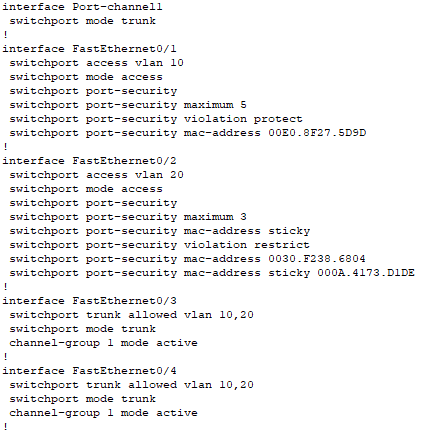
\includegraphics[width=\textwidth,height=\textwidth,keepaspectratio]{./img/lacp/S1.png}
        \caption{Switch 1}
    \end{subfigure}
    \begin{subfigure}{.45\textwidth}
        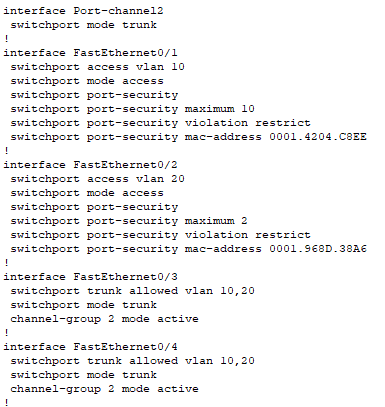
\includegraphics[width=\textwidth,height=\textwidth,keepaspectratio]{./img/lacp/S2.png}
        \caption{Switch 2}
    \end{subfigure}
    ~
    \begin{subfigure}{.45\textwidth}
        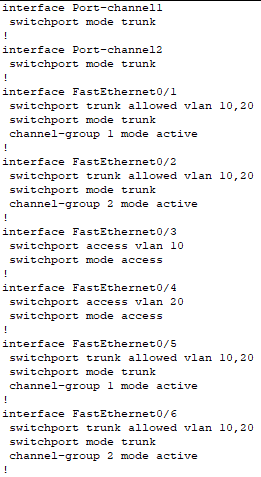
\includegraphics[width=\textwidth,height=\textwidth,keepaspectratio]{./img/lacp/BB.png}
        \caption{Backbone}
    \end{subfigure}
\end{figure}
\begin{figure}[!htb]
    \centering
    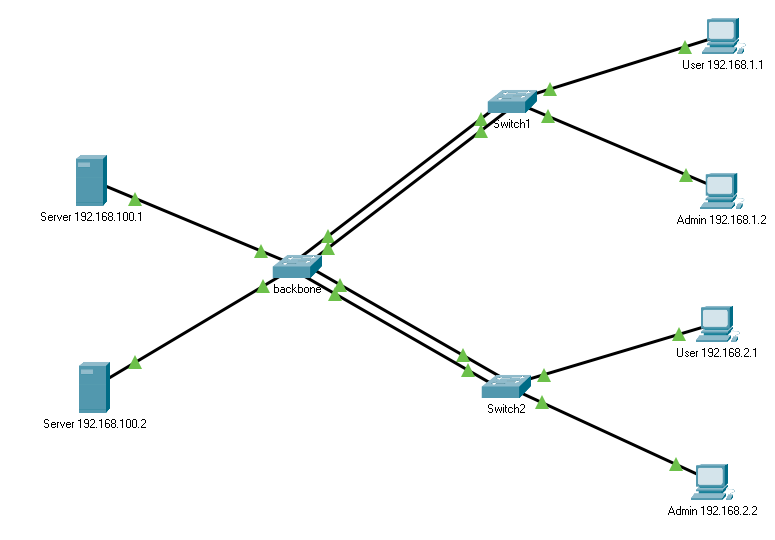
\includegraphics[width=\textwidth,height=\textwidth,keepaspectratio]{./img/lacp/config.png}
    \caption{Aufgebautes Netz mit LACP}
\end{figure}
\FloatBarrier

\subsubsection{FTP Download Resultate}
User 192.168.1.1: 15.246 sec\\
User 192.168.1.2: 15.546 sec\\
Admin 192.168.2.1: 15.256 sec\\
Admin 192.168.2.2: 15.441 sec\\
\begin{figure}[!htb]
    \centering
    \begin{subfigure}{.45\textwidth}
        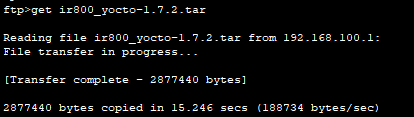
\includegraphics[width=\textwidth,height=\textwidth,keepaspectratio]{./img/lacp/user1.png}
        \caption{User 192.168.1.1}
    \end{subfigure}
    \begin{subfigure}{.45\textwidth}
        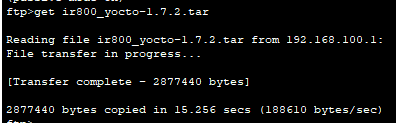
\includegraphics[width=\textwidth,height=\textwidth,keepaspectratio]{./img/lacp/user2.png}
        \caption{User 192.168.1.2}
    \end{subfigure}
    ~
    \begin{subfigure}{.45\textwidth}
        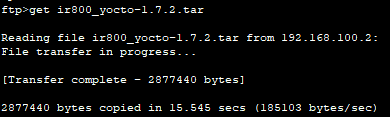
\includegraphics[width=\textwidth,height=\textwidth,keepaspectratio]{./img/lacp/admin1.png}
        \caption{Admin 192.168.2.1}
    \end{subfigure}
    \begin{subfigure}{.45\textwidth}
        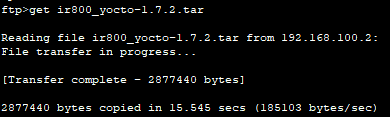
\includegraphics[width=\textwidth,height=\textwidth,keepaspectratio]{./img/lacp/admin1.png}
        \caption{Admin 192.168.2.2}
    \end{subfigure}
\end{figure}
\subsubsection{Frage 6}
\paragraph{Frage}
Warum verdoppelt sich die jetzt erreichte Datenrate nicht, wo liegt das
„Bottleneck“ (die Stelle mit dem geringsten Durchsatz, die die erreichte
Datenrate determiniert)?
\paragraph{Antwort}
Der EtherChannel unterstützt mehrere Load Balancing Methoden und die Werkeinstellungen benutzen die "src-mac forwarding" Methode, was bedeutet, dass Packets von der gleichen Src über den gleichen Port gehen. Damit wirklich die doppelte Datenrate erreicht wird müsste man auf "dest-mac forwarding" umstellen